\documentclass[11pt]{article}
\usepackage[margin=1in]{geometry}
\usepackage{graphicx}
\usepackage{amsmath}
\usepackage{hyperref}

\title{Mini Report: Digital and Control Side of\\
``A 46~\textmu W 13 b 6.4 MS/s SAR ADC With Background Mismatch and Offset Calibration''}
\author{ELEC5705 project notes}
\date{\today}

\begin{document}
\maketitle

\section*{Purpose}
This report isolates the \textbf{digital/control side} of the 2017 JSSC paper by Ding \textit{et al.} and separates it from the full mixed-signal chip implementation. The paper itself is an analog/mixed-signal IC design; it does \textbf{not} discuss FPGA implementation. The useful project angle for an FPGA or HLS mini-project is the background calibration controller that sits around the SAR ADC.

\begin{figure}[h!]
    \centering
    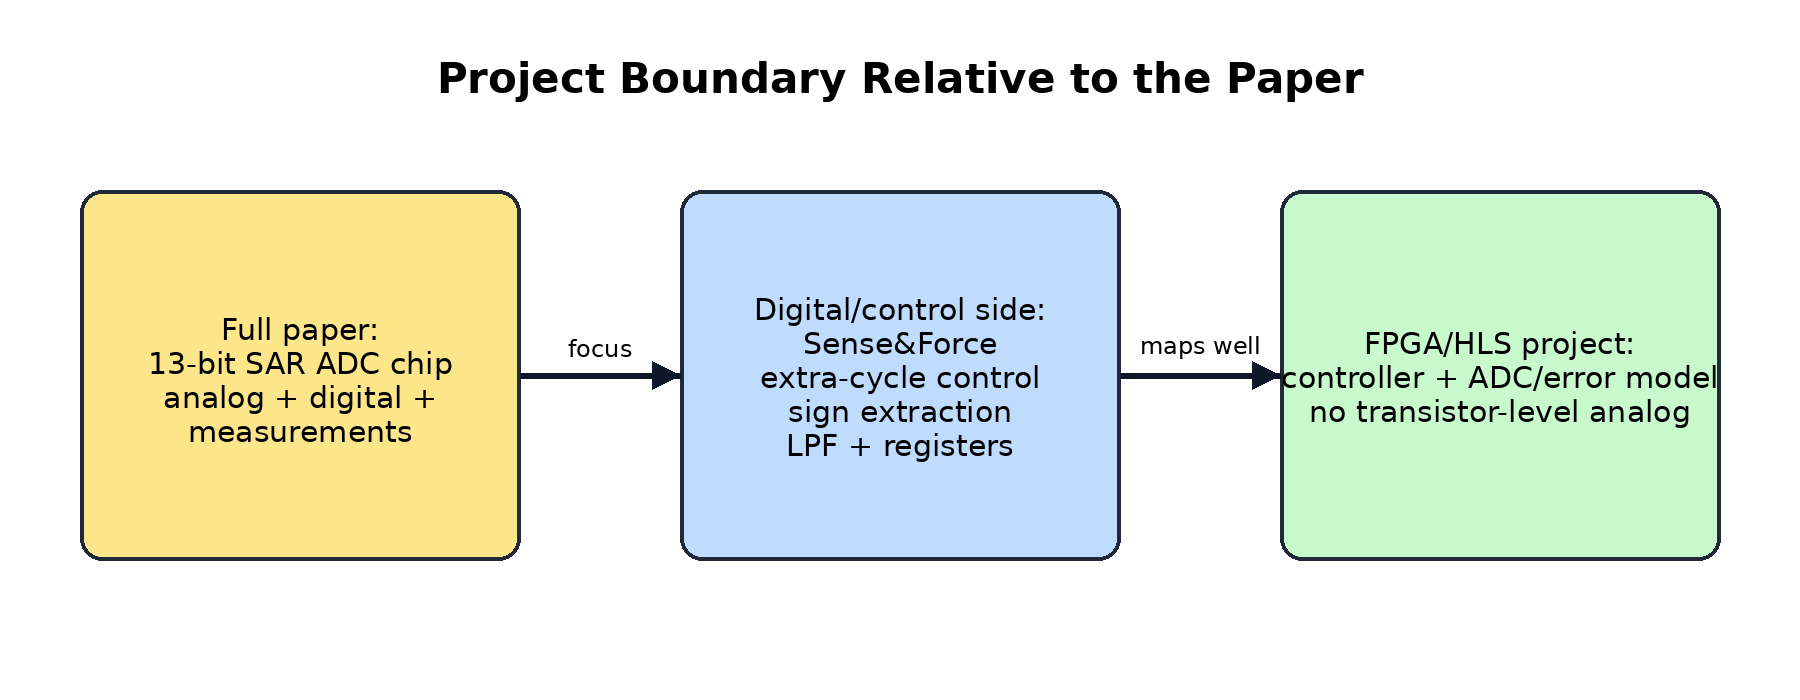
\includegraphics[width=0.95\linewidth]{figures/project_scope.png}
    \caption{Project boundary: the paper is a full mixed-signal ADC chip, while an FPGA/HLS mini-project should focus on the digital calibration controller and a behavioral ADC/error model.}
\end{figure}

\section*{What the Full Paper Contains}
The complete chip contains the following pieces:
\begin{itemize}
    \item a 13-bit SAR ADC with 15 internal comparison cycles and two redundant bits,
    \item a differential capacitive DAC,
    \item a two-mode comparator,
    \item analog correction elements for DAC mismatch and comparator offset,
    \item digital logic that detects error signs and updates calibration settings,
    \item measured silicon validation in 40 nm CMOS.
\end{itemize}

For a digital implementation project, the focus should be the last two items: the \textbf{digital logic that detects when calibration should happen, extracts the sign of the error, filters noisy decisions, and updates calibration registers}.

\section*{Why Redundancy Matters}
The ADC uses 15 raw SAR bits to produce a final 13-bit output. Because of that redundancy, \textbf{different internal raw codes can correspond to the same final output code}. The controller exploits this fact in two ways:
\begin{itemize}
    \item For \textbf{DAC mismatch calibration}, it switches between two redundant internal codes that should ideally produce the same DAC voltage.
    \item For \textbf{comparator offset calibration}, it repeats the final comparison but changes comparator mode.
\end{itemize}

In both cases, the controller does not estimate an exact error magnitude. It only needs the \textbf{sign} of the error so that it can walk a correction word up or down over time.

\section*{Top-Level Digital Calibration Loop}
The digital side is a low-rate adaptive loop wrapped around otherwise normal SAR operation.

\begin{figure}[h!]
    \centering
    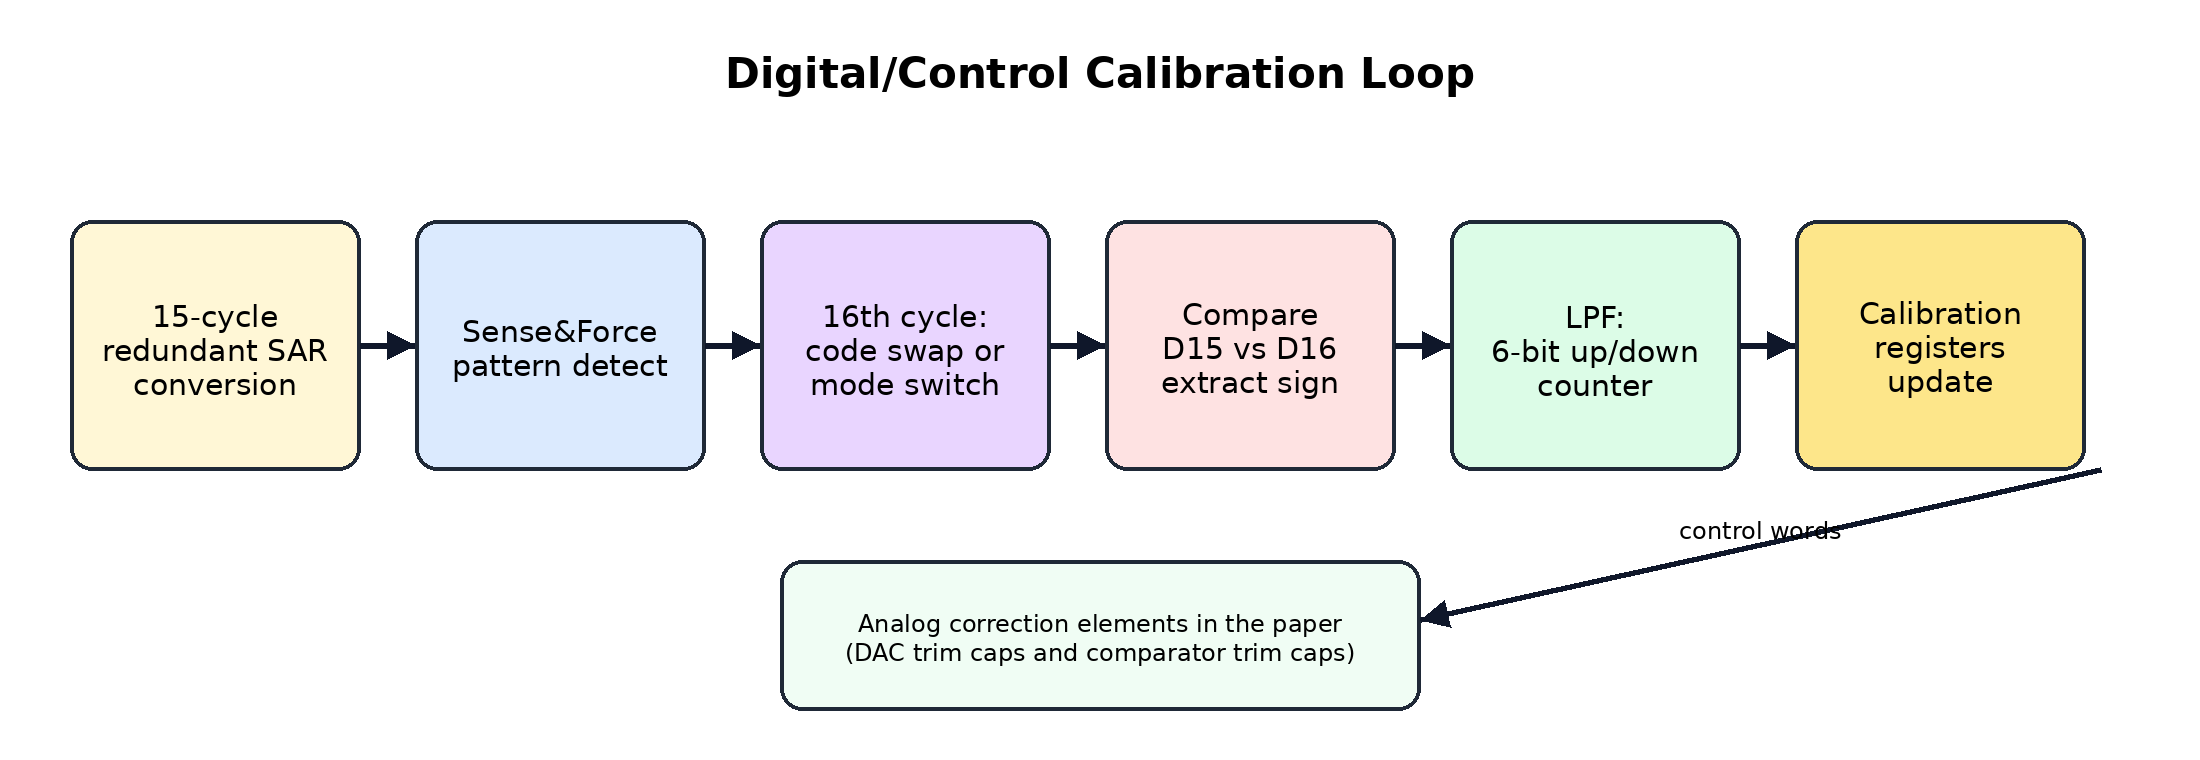
\includegraphics[width=\linewidth]{figures/digital_control_loop.png}
    \caption{High-level digital/control path extracted from the paper. The analog correction elements are in the ASIC, but the detection and update logic is digital and maps well to FPGA/HLS.}
\end{figure}

\noindent The controller performs the following sequence:
\begin{enumerate}
    \item Run the normal 15-cycle redundant SAR conversion.
    \item Monitor the internal raw SAR code for specific trigger patterns.
    \item If a valid pattern appears, enable an extra \(16^{\text{th}}\) cycle.
    \item For DAC calibration, force the alternate redundant code; for comparator calibration, switch comparator mode.
    \item Compare \(D_{15}\) and \(D_{16}\) to obtain the \emph{sign} of the error.
    \item Send that sign through a digital low-pass filter.
    \item Increment or decrement a calibration register only after enough consistent evidence is observed.
\end{enumerate}

\section*{Sense\&Force Logic}
The paper refers to the first control block as \textbf{Sense\&Force}. It continuously monitors the internal 15-bit raw DAC code. The code is partitioned into:
\[
X[6:0], \quad Y[2:0], \quad Z[4:0].
\]

\noindent Calibration is only allowed for very specific patterns so that power consumption stays low. Table~\ref{tab:triggers} summarizes the trigger conditions reported in the paper.

\begin{table}[h!]
\centering
\caption{Calibration trigger patterns used by the controller.}
\label{tab:triggers}
\begin{tabular}{|l|l|c|c|}
\hline
Calibration target & \(X\) pattern & \(Y\) & \(Z\) \\
\hline
MSB & 0111111 / 1000000 & 110 & xxxxx \\
MSB-1 & 0011111 / 0100000 & 110 & xxxxx \\
MSB-2 & 0101111 / 0110000 & 110 & xxxxx \\
MSB-3 & 0110111 / 0111000 & 110 & xxxxx \\
MSB-4 & 0111011 / 0111100 & 110 & xxxxx \\
Comparator & 11000XX & 110 & xxxxx \\
\hline
\end{tabular}
\end{table}

\noindent Why these patterns matter:
\begin{itemize}
    \item They let the controller isolate one calibration event at a time.
    \item The fixed \(Y=110\) condition reduces activation rate and switching activity.
    \item The chosen codes are near the center of the code range, increasing the chance that calibration still happens for non-full-scale inputs.
\end{itemize}

\section*{DAC Mismatch Calibration Flow}
The DAC mismatch calibration is the most FPGA-friendly part of the paper. The controller watches for two \emph{redundant} raw codes \(A\) and \(B\) that should ideally generate the same DAC voltage. If mismatch exists, the two voltages are no longer equal.

\begin{figure}[h!]
    \centering
    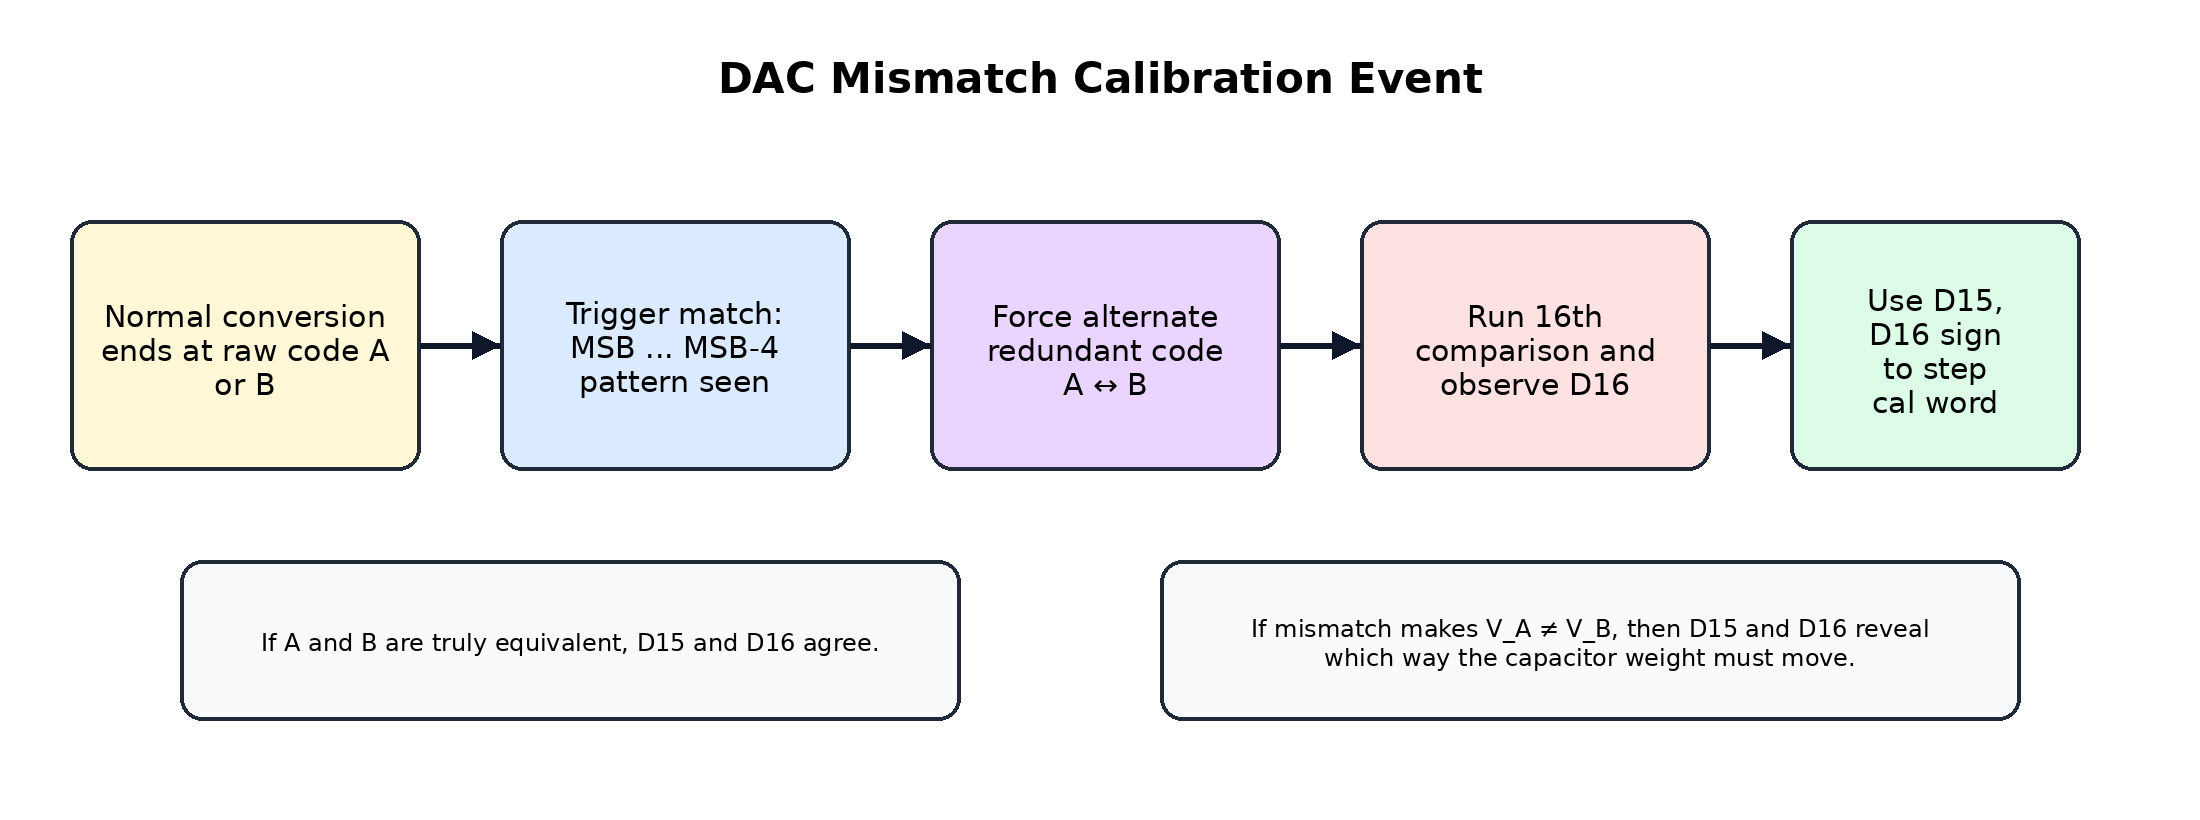
\includegraphics[width=\linewidth]{figures/dac_sequence.png}
    \caption{Controller flow for a DAC calibration event. The paper uses redundancy to create an ``A versus B'' experiment without interrupting normal conversion.}
\end{figure}

\noindent For a triggered capacitor:
\begin{enumerate}
    \item A normal conversion finishes at one redundant code, say \(A\).
    \item The controller enables the extra \(16^{\text{th}}\) comparison.
    \item Sense\&Force swaps the internal code from \(A \leftrightarrow B\).
    \item The comparator produces \(D_{16}\).
    \item The logic compares \(D_{15}\) and \(D_{16}\).
    \item Their difference tells the controller whether \(V_A > V_B\) or \(V_A < V_B\).
    \item That sign becomes an increment or decrement request for the corresponding capacitor trim word.
\end{enumerate}

\noindent The important point is that the controller never solves a full optimization problem. It simply performs a \textbf{signed feedback update}. Over many occurrences of the trigger code, the trim setting converges.

\section*{Comparator Offset Calibration Flow}
The comparator operates in two modes:
\begin{itemize}
    \item low-power mode during coarse decisions,
    \item low-noise mode during fine decisions.
\end{itemize}
Because the two modes do not have identical offset, the controller also runs a background offset calibration. The logic is simpler than the DAC case:
\begin{enumerate}
    \item Finish the normal \(15^{\text{th}}\) comparison.
    \item Keep the DAC code unchanged.
    \item Enable the \(16^{\text{th}}\) cycle and switch comparator mode.
    \item Compare \(D_{15}\) and \(D_{16}\).
    \item Use their difference to determine the sign of the mode-dependent offset error.
    \item Update the comparator correction word after LPF filtering.
\end{enumerate}

\section*{Low-Pass Filter and Register Update Logic}
The paper does not trust every single sign decision, because noise can occasionally flip the comparator result. To avoid reacting to one noisy event, each calibration path includes a digital low-pass filter implemented as a \textbf{6-bit bidirectional counter}.

\begin{figure}[h!]
    \centering
    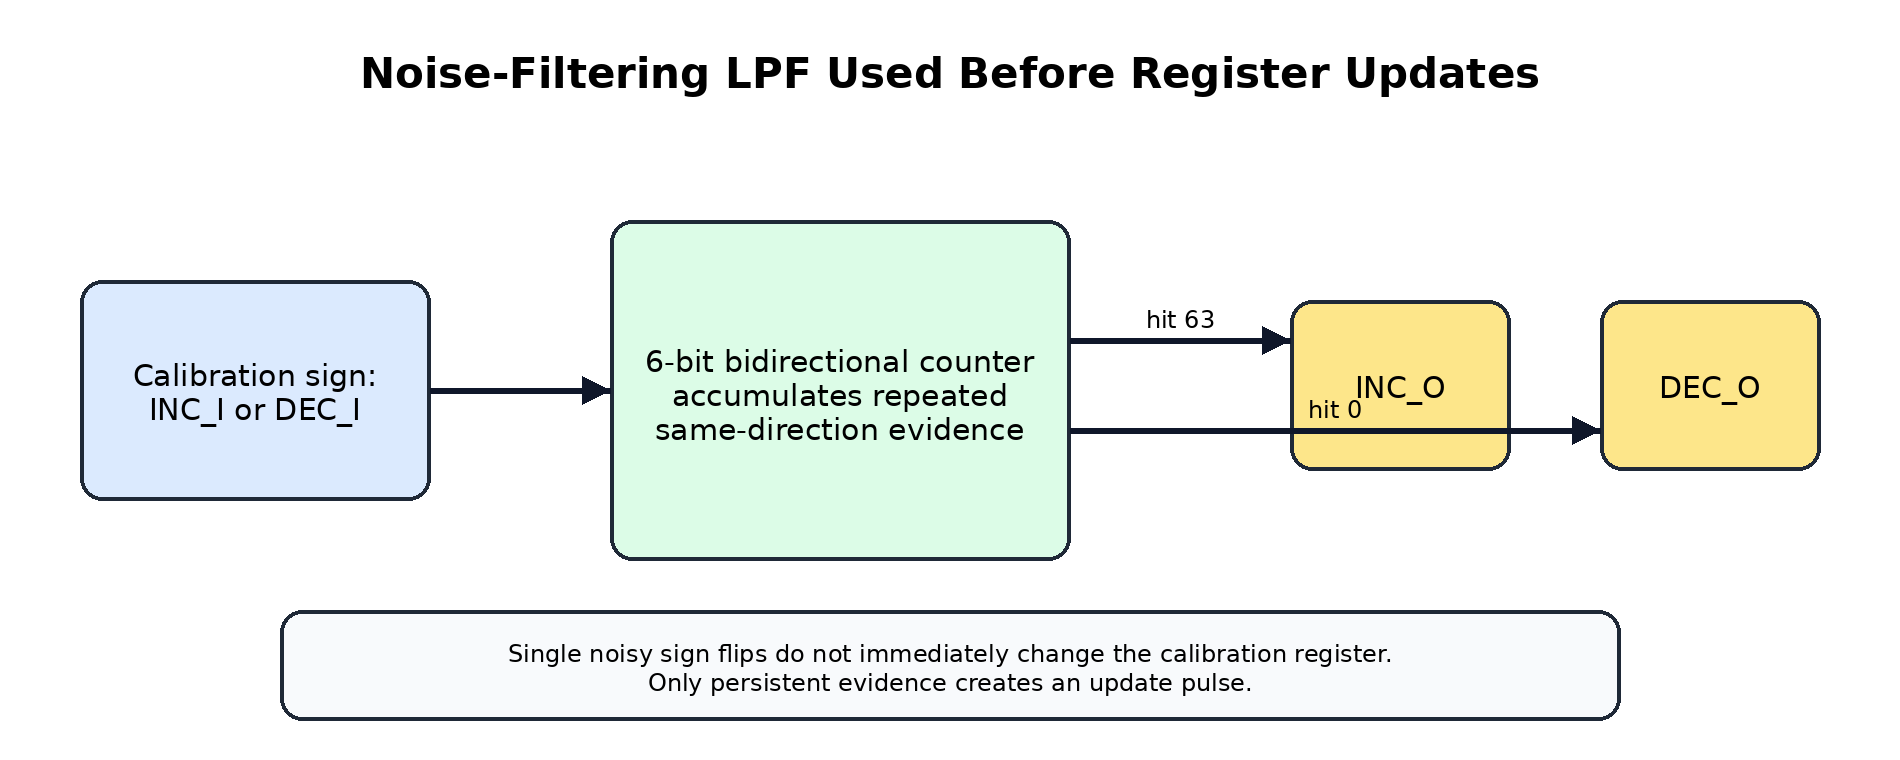
\includegraphics[width=0.92\linewidth]{figures/lpf_counter.png}
    \caption{Digital LPF behavior. Repeated same-direction evidence eventually causes an update pulse; isolated noise events do not.}
\end{figure}

\noindent Its operation is:
\begin{itemize}
    \item If the new evidence says ``increase correction,'' the counter moves up.
    \item If the new evidence says ``decrease correction,'' the counter moves down.
    \item If the count reaches its upper bound, it emits an \(INC\_O\) pulse.
    \item If the count reaches zero, it emits a \(DEC\_O\) pulse.
    \item Only those pulses modify the actual calibration register.
\end{itemize}

\noindent This turns noisy sign samples into a slower, more reliable register update stream.

\section*{Why the Logic Is Low Power}
The digital controller is intentionally lightweight:
\begin{itemize}
    \item It processes only \textbf{sign} information rather than full-precision error values.
    \item It avoids multipliers, LMS blocks, and digital post-correction engines.
    \item It triggers calibration only for rare internal code patterns.
    \item It gates unnecessary activity in the detection logic.
\end{itemize}

The paper reports that the calibration overhead is small enough that total calibration power is about \(5\%\) of the ADC power budget.

\section*{How the Paper Shows It Works}
The authors validate the controller at three levels:
\begin{enumerate}
    \item \textbf{MATLAB Monte Carlo simulations}: show that the calibrated design can use much smaller unit capacitors while still meeting linearity targets.
    \item \textbf{Circuit-level integrated simulations}: show improved SNDR and INL after the calibration loops are enabled.
    \item \textbf{Measured silicon results}: show lower INL/DNL error, about 20 dB spur suppression, and roughly 400k cycles to settle after calibration is enabled.
\end{enumerate}

\begin{figure}[h!]
    \centering
    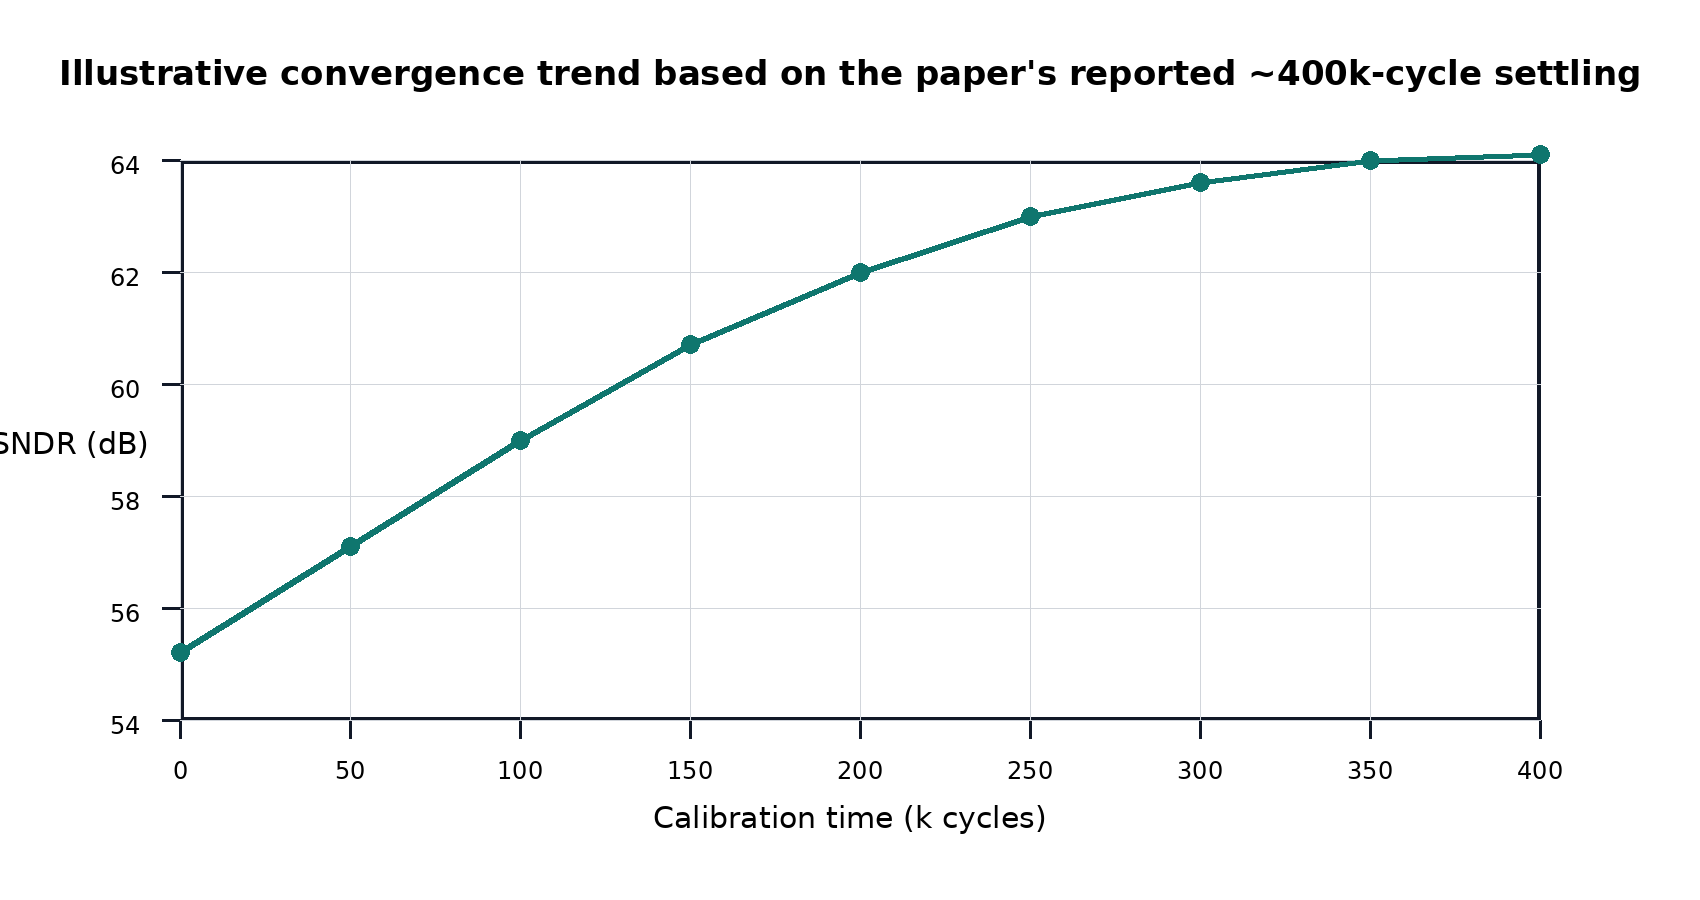
\includegraphics[width=0.84\linewidth]{figures/convergence_trend.png}
    \caption{Illustrative convergence trend aligned to the paper's reported \(\sim 400\)k-cycle settling time.}
\end{figure}

\section*{What Maps Cleanly to FPGA or HLS}
The following parts of the paper map directly to an HLS mini-project:
\begin{itemize}
    \item internal-code trigger detection,
    \item extra-cycle scheduler,
    \item DAC code swap controller,
    \item comparator-mode swap controller,
    \item \(D_{15}\) versus \(D_{16}\) sign extraction,
    \item LPF counters,
    \item calibration registers.
\end{itemize}

\noindent The following parts \emph{do not} map directly to FPGA:
\begin{itemize}
    \item physical capacitor mismatch,
    \item analog comparator circuits,
    \item capacitive trim arrays,
    \item transistor-level low-power design.
\end{itemize}

\noindent Therefore, a sensible FPGA project is:
\begin{quote}
Implement the sign-based background calibration controller in HLS and connect it to a behavioral model of a redundant SAR ADC with DAC mismatch and optional comparator offset.
\end{quote}

\section*{Conclusion}
The digital/control contribution of the paper is a compact background calibration engine that:
\begin{itemize}
    \item detects \emph{when} an internal raw SAR code is useful for calibration,
    \item inserts an extra calibration comparison,
    \item extracts only the \emph{sign} of DAC mismatch or comparator offset error,
    \item filters noisy decisions with a bidirectional-counter LPF,
    \item updates calibration registers that steer analog correction hardware.
\end{itemize}

\noindent That controller, rather than the full ADC ASIC, is the part worth isolating for an FPGA/HLS course project.

\vfill
\noindent\textbf{Primary source:}
M. Ding, P. Harpe, Y.-H. Liu, B. Busze, K. Philips, and H. de Groot, ``A 46~\textmu W 13 b 6.4 MS/s SAR ADC With Background Mismatch and Offset Calibration,'' \emph{IEEE Journal of Solid-State Circuits}, vol. 52, no. 2, Feb. 2017.

\end{document}
